	%% This is file `elsarticle-template-1-num.tex',
%%
%% Copyright 2009 Elsevier Ltd
%%
%% This file is part of the 'Elsarticle Bundle'.
%% ---------------------------------------------

\documentclass[a4paper]{article}

%% Use the option review to obtain double line spacing
%% \documentclass[preprint,review,12pt]{elsarticle}

%% Use the options 1p,twocolumn; 3p; 3p,twocolumn; 5p; or 5p,twocolumn
%% for a journal layout:
%% \documentclass[final,1p,times]{elsarticle}
%% \documentclass[final,1p,times,twocolumn]{elsarticle}
%% \documentclass[final,3p,times]{elsarticle}
%% \documentclass[final,3p,times,twocolumn]{elsarticle}
%% \documentclass[final,5p,times]{elsarticle}
%% \documentclass[final,5p,times,twocolumn]{elsarticle}

%% The graphicx package provides the includegraphics command.
\usepackage{graphicx}
\usepackage{import}
\usepackage{xifthen}
\usepackage{pdfpages}
\usepackage{transparent}
\usepackage{cancel}
%% The amssymb package provides various useful mathematical symbols
\usepackage{amssymb}
\usepackage{amsmath}
\usepackage{bm}
\usepackage{amsthm}
\usepackage{ mathrsfs }
\usepackage{ dsfont }
\usepackage{tikz-cd}
\usepackage[a4paper,top=3cm,bottom=2cm,left=3cm,right=3cm,marginparwidth=1.75cm]{geometry}
\usepackage{float}
%% The lineno packages adds line numbers. Start line numbering with
%% \begin{linenumbers}, end it with \end{linenumbers}. Or switch it on
%% for the whole article with \linenumbers after \end{frontmatter}.
\usepackage{lineno}
\usepackage{hyperref}
\usepackage{enumitem}
\usepackage{tikz}
\usetikzlibrary{positioning,calc}
%% natbib.sty is loaded by default. However, natbib options can be
%% provided with \biboptions{...} command. Following options are
%% valid:

%%   round  -  round parentheses are used (default)
%%   square -  square brackets are used   [option]
%%   curly  -  curly braces are used      {option}
%%   angle  -  angle brackets are used    <option>
%%   semicolon  -  multiple citations separated by semi-colon
%%   colon  - same as semicolon, an earlier confusion
%%   comma  -  separated by comma
%%   numbers-  selects numerical citations
%%   super  -  numerical citations as superscripts
%%   sort   -  sorts multiple citations according to order in ref. list
%%   sort&compress   -  like sort, but also compresses numerical citations
%%   compress - compresses without sorting
%%
%% \biboptions{comma,round}

% \biboptions{}
\newtheorem{name}{Printed output}
\newtheorem{mydef}{Definition}
\newtheoremstyle{break}% name
  {}%         Space above, empty = `usual value'
  {}%         Space below
  {}%         Body font
  {}%         Indent amount (empty = no indent, \parindent = para indent)
  {\bfseries}% Thm head font
  {.}%        Punctuation after thm head
  {\newline}% Space after thm head: \newline = linebreak
  {}%         Thm head spec

\theoremstyle{plain} %italics
\newtheorem{question}{Question}

\newtheorem{theorem}{Theorem}[section]
%\numberwithin{theorem}{subsection}

\newtheorem*{lemma*}{Lemma}
\newtheorem{lemma}[theorem]{Lemma}
%\numberwithin{lemma}{subsection}

\newtheorem{corollary}[theorem]{Corollary}
%\numberwithin{corollary}{subsection}

\newtheorem{proposition}[theorem]{Proposition}
%\numberwithin{proposition}{subsection}

\theoremstyle{definition} %non italics

\newtheorem{definition}[theorem]{Definition}
%\numberwithin{definition}{subsection}

\newtheorem{algorithm}{Algorithm}

\newtheorem*{note*}{Note}

\newtheorem*{claim}{Claim}

\newtheorem*{remark}{Remark}

\newtheorem*{example}{Example}

\numberwithin{equation}{subsection}

\newcommand{\incfig}[1]{%
    \def\svgwidth{\columnwidth}
    \import{./figures/}{#1.pdf_tex}
}
\newcommand{\hodge}{{*}}
\newcommand{\tang}{\operatorname{\textbf{\textup{t}}}}
\newcommand{\norm}{\operatorname{\textbf{\textup{n}}}}
%mathbb short cut
\newcommand{\R}{\mathbb{R}}
\newcommand{\bP}{\mathbb{bP}}
\newcommand{\N}{\mathbb{N}}
\newcommand{\Q}{\mathbb{Q}}
\newcommand{\A}{\mathbb{A}}
\newcommand{\bS}{\mathbb{S}}
\newcommand{\Z}{\mathbb{Z}}
\newcommand{\F}{\mathbb{F}}
\newcommand{\B}{\mathbb{B}}
\newcommand{\T}{\mathbb{T}}
\newcommand{\K}{\mathbb{K}}
\newcommand{\C}{\mathbb{C}}
\newcommand{\D}{\mathbb{D}}

\usepackage{comment}
\setlength{\parindent}{0pt}    % no indentation
\setlength{\parskip}{1em}      % add vertical space between paragraphs
%bm short cut
\newcommand{\bmv}{\bm{v}}
\newcommand{\bmu}{\bm{u}}
\newcommand{\bmw}{\bm{w}}
\newcommand{\bmx}{\bm{x}}

%mathcal shortcut
\newcommand{\cF}{\mathcal{F}}
\newcommand{\cA}{\mathcal{A}}
\newcommand{\cM}{\mathcal{M}}
\newcommand{\cU}{\mathcal{U}}
\newcommand{\cB}{\mathcal{B}}
\newcommand{\cD}{\mathcal{D}}
\newcommand{\cL}{\mathcal{L}}
\newcommand{\cS}{\mathcal{S}}
\newcommand{\cG}{\mathcal{G}}
\newcommand{\cT}{\mathcal{T}}
\newcommand{\cC}{\mathcal{C}}
\newcommand{\cH}{\mathcal{H}}
\newcommand{\cO}{\mathcal{O}}
\newcommand{\cJ}{\mathcal{J}}

%mathfraktur shortcut
\newcommand{\frp}{\mathfrak{p}}
\newcommand{\frq}{\mathfrak{q}}
\newcommand{\frm}{\mathfrak{m}}
\newcommand{\frP}{\mathfrak{P}}

%mathscr shortcut
\newcommand{\msF}{\mathscr{F}}
\newcommand{\msA}{\mathscr{A}}
\newcommand{\msM}{\mathscr{M}}
\newcommand{\msE}{\mathscr{E}}
\newcommand{\msU}{\mathscr{U}}
\newcommand{\msB}{\mathscr{B}}
\newcommand{\msD}{\mathscr{D}}
\newcommand{\msL}{\mathscr{L}}
\newcommand{\msS}{\mathscr{S}}
\newcommand{\msG}{\mathscr{G}}
\newcommand{\msT}{\mathscr{T}}
\newcommand{\msC}{\mathscr{C}}
\newcommand{\msH}{\mathscr{H}}
\newcommand{\msO}{\mathscr{O}}
\newcommand{\msJ}{\mathscr{J}}
\newcommand{\msP}{\mathscr{P}}


%set notation shortcut
\newcommand{\vect}[1]{\underline{\textbf{#1}}}
\newcommand{\llangle}{\left\langle}
\newcommand{\rrangle}{\right\rangle}
\newcommand{\llbrace}{\left\lbrace}
\newcommand{\rrbrace}{\right\rbrace}
\newcommand{\setof}[1]{\left\lbrace #1 \right\rbrace}


\newcommand{\cFA}{\cF(\cA)}
\newcommand{\sigmaA}{\sigma(\cA)}
\newcommand{\del}[2]{\frac{\partial #1}{\partial #2}}


\newcommand{\innerproductb}[2]{\llangle\bm{#1},\bm{#2}\rrangle}
\newcommand{\innerproduct}[2]{\llangle{#1},{#2}\rrangle}

\newcommand{\cl}{\operatorname{cl}}
\newcommand{\coker}{\operatorname{coker}}
\newcommand{\re}{\operatorname{Re}}
\newcommand{\im}{\operatorname{Im}}
\newcommand{\dist}{\operatorname{dist}}
\newcommand{\Span}{\operatorname{Span}}
\newcommand{\Supp}{\operatorname{Supp}}
\newcommand{\id}{\operatorname{id}}
\newcommand{\sh}{\operatorname{sh}}
\newcommand{\var}{\operatorname{Var}}
\newcommand{\Proj}{\operatorname{Proj}}
\newcommand{\Ker}{\operatorname{Ker}}
\newcommand{\Mor}{\operatorname{Mor}}
\newcommand{\supp}{\operatorname{supp}}
\newcommand{\Ran}{\operatorname{Ran}}
\newcommand{\Res}{\operatorname{Res}}
\newcommand{\Mod}{\operatorname{Mod}}
\newcommand{\res}{\operatorname{res}}
\newcommand{\Frac}{\operatorname{Frac}}
\newcommand{\End}{\operatorname{End}}
\newcommand{\Sym}{\operatorname{Sym}}
\newcommand{\Spec}{\operatorname{Spec}}
\newcommand*{\sheafhom}{\mathcal{H}\kern -.5pt \it{ om}}
\newcommand*{\sheafspec}{\mathcal{S}\kern -.5pt \it{ pec}}
\newcommand*{\sheafproj}{{\mathcal{P}\kern -.5pt \it{ roj}}}
\newcommand{\Div}{\operatorname{div}}
\newcommand{\Aut}{\operatorname{Aut}}
\newcommand{\Hom}{\operatorname{Hom}}
\newcommand{\Qcoh}{\operatorname{Qcoh}}
\newcommand{\PGL}{\operatorname{PGL}}
\newcommand{\Op}{\operatorname{Op}}
\newcommand{\WF}{\operatorname{WF}}
\newcommand{\Char}{\operatorname{Char}}
\newcommand{\Ell}{\operatorname{Ell}}
\newcommand{\RE}{\operatorname{Re}}
\newcommand{\IM}{\operatorname{Im}}

\newcommand{\vx}{{\textbf{x}}}
\newcommand{\vy}{{\textbf{y}}}
\newcommand{\vz}{{\textbf{z}}}
\newcommand{\vw}{{\textbf{w}}}
\newcommand{\va}{{\textbf{a}}}
\newcommand{\vb}{{\textbf{b}}}
% \usepackage{bm} % make sure this is in your preamble
\newcommand{\vsigma}{{\bm{\sigma}}} % bold sigma (math)

\newcommand{\vxh}{{\widehat{\textbf{x}}}}
\newcommand{\vyh}{{\widehat{\textbf{y}}}}
\newcommand{\Xh}{{\widehat{X}}}
\newcommand{\Yh}{{\widehat{Y}}}

\begin{document}

%% Title, authors and addresses

\title{\textbf{Deep Neural Networks via Tensor Calculus}}

%% use the tnoteref command within \title for footnotes;
%% use the tnotetext command for the associated footnote;
%% use the fnref command within \author or \address for footnotes;
%% use the fntext command for the associated footnote;
%% use the corref command within \author for corresponding author footnotes;
%% use the cortext command for the associated footnote;
%% use the ead command for the email address,
%% and the form \ead[url] for the home page:
%%
%% \title{Title\tnoteref{label1}}
%% \tnotetext[label1]{}
%% \author{Name\corref{cor1}\fnref{label2}}
%% \ead{email address}
%% \ead[url]{home page}
%% \fntext[label2]{}
%% \cortext[cor1]{}
%% \address{Address\fnref{label3}}
%% \fntext[label3]{}


%% use optional labels to link authors explicitly to addresses:
%% \author[label1,label2]{<author name>}
%% \address[label1]{<address>}
%% \address[label2]{<address>}

\author{\textbf{Jeffrey Thompson}}
\maketitle
\begin{abstract}
This is my experience with deriving and implementing a fully custom neural network framework. 
The goal of this write-up is to slowly introduce technical mathematical language and concepts chronologically 
so that an arbitrary reader can gain some value by reading up to where they can no longer follow. Once reaching this point, 
an interested reader should have the tools to further explore any concepts presented here and revisit at a later point.

This framework was implemented in Python here: \url{https://github.com/Jaffulee/deep_neural_network}
\end{abstract}
\tableofcontents
\newpage
\section{Overview and Motivation}
The first question is: what do we want to achieve?

\subsection{The Goal}
The goal is to solve complex non-linear problems (in finite dimensions).

Linear problems are those where scaling the input also scales the output by a similar amount. 
For example, if an apple costs £$1$, then 5 apples at that price will cost £$5$. 
Linear problems are easy to solve! 

Most interesting problems, however, are highly non-linear. 
For example, given the camera feed from a self-driving car, how can we use that data to steer the car in a sensible direction?

The trouble with non-linear problems is that there may not be a nice way to solve them analytically, and thus we must turn to numeric schemes.

Additionally, in the real world, we often only have a sample of data to work with, and would like to find a way to consistently map the input data to the desired output data.

So more specifically, we would like a way to take samples of inputs, and form a way of non-linearly combining the input data so that we can solve some problem.

\subsection{The Setup to the Problem} \label{sec:the-setup-to-the-problem}

We are given a dataset $\mathcal{D}$ of $m$ input-output pairs of real-valued vectors $(\vxh_{(i)}, \vyh_{(i)})$; 
\[
\mathcal{D} = \{(\vxh_{(i)}, \vyh_{(i)}) \mid \vxh_{(i)} \in \R^{n_x}, \; \vyh_{(i)} \in \R^{n_y}, \; i=1,\dots,m \}.
\]
Here $n_x$ denotes the number of \emph{input features} (the dimension of each state), and 
$n_y$ denotes the number of \emph{output features} (the dimension of each target).
\begin{example}
  
  In the setup of a self-driving racecar, we might use training data of human drivers on a racetrack, 
  and we could collect input data such as the distance to the side of the road, 
  the angle of the car, the speed and acceleration of the car, etc. in our $\vxh$ vector, with one entry per measurement, 
  and $n_x$ is the number of entries.
  The outputs collected could then be the decision the driver made such as steering right, braking, accelerating, etc. collected in our $\vyh$ vector, 
  and $n_y$ is the number of decisions. 
  Our number of input-output pairs, $m$, will be very large in this scenario, since we might be collecting data every few milliseconds, for many laps.
\end{example}
We want to produce a function $\vy = \vy(\vx)$ which takes $\vx$ as an input such that $\vy(\vxh_{i}) \approx \vyh_{i}$. 
We also want to be able to input $\vx$ values which are not from $\vxh$, and would like these unknown inputs to produce reasonable results.

\begin{example}
  In our racecar example, we cannot possibly record enough data to cover every possible input on the racetrack, so we need to be able to reasonably interpolate between the observed values, and be able to make a decision from the output vector similar to what a real driver would do.
\end{example}

\begin{example}
  Let's say we have a business which helps customers decide whether their fruit is an apple or a pear,
  based on the colour (average hue), and the roundness (e.g. height - length).
  $\vxh$ will be a vector of (colour, roundness) and therefore $n_x = 2$, 
  and $\vyh$ will be a vector which indicates either of (apple, pear), hence $n_y = 2$.
  From this, we have two actions: the fruit is an apple or it is a pear.
  Let's say, as a business, we have produced a mystical function which takes in (red, round), and outputs $(0.99, 1)$. 
  We can interpret this as our mystical function is $99\%$ sure that the input results in a value of apple.
\end{example}
How do we find such a function $\vy$?
\newpage
\section{Gradient Descent}
\subsection{A Brief Dip into Calculus}

If $f:\R \rightarrow \R ; \; x \mapsto f(x)$ is a \emph{function which smoothly takes real numbers to real numbers} (e.g. $f(x) = 2x$), 
we can consider the \emph{slope of $f$ between two points} to be
\begin{equation} \label{eq:derivative-first-principals}
  \frac{\Delta f}{\Delta x}
\end{equation}

The delta $\Delta$ represents a \emph{small change}; this is the change in f divided by the change in x. 
If we make the change infinitely small (and repeat this for all values of $x$), we get \emph{the gradient of f at the point $x$}, denoted by
\[ \frac{df}{dx} \]

It turns out finding the gradient of a lot of functions is relatively simple, by (rigorously) making the small change in Equation \ref{eq:derivative-first-principals} become 0. If we briefly drop rigor\footnote{The presented division works whenever $\Delta f$ is not 0 near to $x$, and some more work is needed to make this intuition rigorous, especially around the exchanging of limits and multiplication. Nevertheless, it neatly gives an intuitive foundation for the chain rule.}
, and define a composite function $g = g(f(x))$, and since (again non-rigorously) $\Delta f / \Delta f = 1$, we can compute:
\[ \frac{\Delta g}{\Delta x} = \frac{\Delta g}{\Delta f} \frac{\Delta f}{\Delta x}\]

Making the change infinitely small (up to rigor), gives us:
\begin{theorem} \label{th:chain-rule-1d}
  The Chain Rule:

  If $f, \; g : \R \rightarrow \R $ are suitably smooth and defined, then the composition $g(f(x))$ has the gradient:
  \[\frac{dg}{dx} = \frac{dg}{df}\frac{df}{dx}\]
\end{theorem}

This is an essential Theorem, since it means that we can calculate the gradient of very complex functions as long as we can write that function as a sequence of simpler functions.

\subsection{Gradient Descent Motivation}

A key fact is that the value of the gradient of a function $f$ at $x$ points in the $x$-direction of steepest ascent of the function, i.e. where we should move $x$ to increase $f$ by the most. This means if we move $x$ in the direction of the gradient of the function at that point, we can always move in the direction where the function is increasing.
Similarly, if we move in the opposite direction, we can move in the direction where the function is decreasing the most.

This is an essential part of how we will construct our $\vy$ function from before in Section \ref{sec:the-setup-to-the-problem}; if we have a function that tells us how far away from the correct answer we are, an error or loss function, we can find where the 
error is smallest by moving $x$ in the direction where the error is decreasing. This can be thought of like rolling a ball down a hill until it reaches the bottom. Unfortunately, there is an issue with this method: 
if the hill is curvy enough, our ball might get stuck in a ditch that is not the bottom of the hill. We can ``fix'' this issue by starting with our ball at random parts of the hill, seeing where it rolls down to, and making note of the one that got the lowest.

This concept is the idea behind gradient descent: we want a function $E$ 
which takes in some number of inputs, and outputs an \emph{error/loss/cost} as a number in which 0 represents the best. Since 0 is the minimum of $E$, finding the inputs that result in the least error/loss/cost amounts to finding a global minimum. 
This is very similar to the scenario above; we can try to utilise gradient descent.

\subsection{Gradient Descent in 1 Dimension}

Formulating gradient descent amounts to writing our intuition out accurately.

\begin{theorem} \label{th:gradient-descent-1d}
  Gradient Descent 1D

  Let $E:\R \rightarrow \R^+$ be a non-negative real-valued function which is sufficiently smooth
  and let $\alpha \in (0,1]$ be a number between zero and one called the learning rate. 
  Let $x_n$ be a sequence of real numbers defined by the iterative process:
  \[ x_{n+1} = x_n - \alpha \frac{dE}{dx}\bigg|_{x=x_n}\]

  Where the bar denotes evaluating the gradient at the point $x_n$. Then, for an appropriately small $\alpha$,\footnote{The convergence of this process utilises that the derivative's magnitude is roughly proportional to how far we are from a local minimum. If $\alpha$ is too large, we may continually overshoot the minumum to where the magnitude of the gradient has not decreased. This would cause us to not converge.} 
  $x_n$ approaches a local minimum or a turning point of $E$ as $n$ increases.
\end{theorem}

By looking at the equation above, one can see that if $\frac{dE}{dx}\big|_{x=x_n}$ is very small (similarly if $\alpha$ is very small), $x_{n+1} \approx x_n$.
Points where $\frac{dE}{dx}=0$ are called turning points, and thus we have justified the final sentence of Theorem \ref{th:gradient-descent-1d}. 
The problem we face is that turning points are not necessarily minima; we would like to avoid landing on non-minima turning points.

There are various methods to adapt gradient descent to improve the issue of turning points. One approach is to include momentum. 
Continuing with the ball rolling analogy for gradient descent, we can mimic momentum by calculating the speed at which $x$ itself is moving, 
and adding that to our formula. This allows for the ball to roll past turning points using the speed it had to reach it.

Momentum can still run into an issue of if the ball perfectly landed on a turning point with no momentum, it can still get stuck. 
To account for this, we can include an additional force to push the ball every once in a while. This can be thought of as a random gust of wind.

\begin{theorem} \label{th:gradient-descent-1d-mom-wind}
  Gradient Descent with Momentum and Wind (Noise)
  
  Let $E:\R \rightarrow \R^+$ be a non-negative real-valued function which is sufficiently smooth
  and let $\alpha, \; \beta \in (0,1]$ be numbers between zero and one called the learning rate and the momentum parameter respectively. 
  Let $\gamma$ be a random number centered around 0, and let $g: \N \rightarrow \R; \; g: n \mapsto g(n)$ be a real-valued function of 
  the current iteration called the noise parameter.
  Let $x_n$ be a sequence of real numbers defined by the iterative process:
  \[ x_{n+1} = x_n - \alpha \frac{dE}{dx}\bigg|_{x=x_n} - \beta (x_{n} - x_{n-1}) + g(n)\gamma \]

  Where the bar denotes evaluating the gradient at the point $x_n$. Then, for an appropriate choice of $\alpha, \; \beta, \; g$,
  we have that $x_n$ approaches a local minimum of $E$ as $n$ increases.

  The parameters $\alpha, \; \beta, \; g$ are referred to as hyperparameters\footnote{The word hyper is used here since we are looking at gradient descent from the point of view of a neural network, where the gradient descent parameters are seen as pre-chosen. Choosing appropriate hyperparameters can be difficult.}.
\end{theorem}

The selection we will make for here $g(n)$ is usually 1 when $n$ is some multiple of a number and 0 otherwise - a burst of noise every fixed number of iterations - and our choice 
of $\gamma$ will be usually a normal distribution with mean zero and variance a fixed number.

The learning rate $\alpha$ roughly corresponds to ``smaller is more accurate but slower, larger is less accurate but quicker'', and the momentum parameter $\beta$ can be thought of as the mass of our rolling ball, and $1$ represents infinite mass.

The great news is that gradient descent in Theorem \ref{th:gradient-descent-1d-mom-wind} only really depends on the gradient at a point, and storing some extra previous or random numbers. 
This makes it quite simple to implement in code, as long as you have a sensible way of getting the gradient.

\subsection{A Brief Dip into Multi-Variable Calculus}

We care about vectors due to our setup of the problem in Section \ref{sec:the-setup-to-the-problem}. What if a function depends on a vector, i.e. what if it has many input variables $f = f(x^1, \dots, x^n)$? 
Note that the superscript is just indexing the argument component\footnote{Superscripts for indexing vectors is a convention utilised in differential geometry which helps with book-keeping later.}, 
not taking a number to a power.
We want a way of seeing how $f$ changes with respect to its input variables. For convenience, let us write $f = f(\vx)$, where $\vx = (x^1, \dots, x^n)^T$.
Note $T$ denotes \emph{transposing} so that $\vx$ is a column vector.

We can reuse our notion of a gradient for a function with one variable from Equation \ref{eq:derivative-first-principals} by fixing all but one of the $x^i$s,
and computing the gradient of the remaining $x^i$ as before. To distinguish this process from the one-variable process, we call this a \emph{partial derivative of $f$ with respect to $x^i$} and denote it with ``del'', a curly d:
\[ \del{f}{x^i} \]

Now we can reuse our notion of a gradient by calculating the partial derivative with respect to each $x^i$ in $\vx$ separately.
\begin{definition} \label{def:grad-f}
  The gradient of a function with multiple variables.

  Define the gradient of $f = f(\vx)$, denoted $\nabla_\vx f$ to be:
  \[
  \nabla_\vx f = \left( \del{f}{x^1}, \dots, \del{f}{x^n}  \right)^T
  \] 
\end{definition}

Importantly, the gradient still points in the direction of steepest ascent of $f$ with respect to the input variables $\vx$.
Thus, we can extend gradient descent to a function of multiple variables by conducting gradient descent on each component.

Before doing this, we also need to introduce the concept of a gradient when we have nested functions. Let's say that each $x^i$ is itself a function of $m$ variables, 
i.e. $\vx = \vx(\textbf{w})$, where $\textbf{w} = (w^1, \dots, w^m)^T$:

We would like to know how $f$ changes when one of the $w^i$ changes.

\[
\vx = \vx(\textbf{w}) = \begin{bmatrix}
  x^1(\textbf{w}) \\
  x^2(\textbf{w}) \\
  \vdots \\
  x^n(\textbf{w})
\end{bmatrix} = \begin{bmatrix}
  x^1(w^1, \dots, w^m) \\
  x^2(w^1, \dots, w^m) \\
  \vdots \\
  x^n(w^1, \dots, w^m)
\end{bmatrix}
\]

\begin{definition} \label{def:chain-rule-total-derivative}
  Chain Rule for Multi-Variate Functions

  Let $f = f(\vx)$ be a function of $n$ variables, where each variable is a function of m variables $\textbf{w}$, i.e. $\vx = \vx(\textbf{w})$. 
  We can write $f = f(\vx(\textbf{w}))$. Then we define the partial derivative of $f$ with respect to $w^i$, denoted $\del{f}{w^i}$, is the following:
  \[ \del{f}{w^i} = \del{f}{x^1} \del{x^1}{w^i} + \dots + \del{f}{x^n} \del{x^n}{w^i}\]
\end{definition}

Which can be thought of like ``looking at how $f$ changes as you nudge each variable of $f$ by a little bit in one direction.'' Note that this is not quite the previous chain rule, and justifying this definition takes a little more work for the interested reader.

\subsection{Gradient Descent in $n$ Dimensions}

Extending gradient descent to $n$ dimensions, it is mostly an exercise in notation. If $\alpha$ is a real number, and 
$\vx = (x^1,\dots,x^n)^T$ is a vector, we define $\alpha \vx$ to be component-wise multiplication by $\alpha$, 
\[\alpha \vx = (\alpha x^1,\dots,\alpha x^n)^T\]

If $\vy = (y^1, \dots, y^n)^T$ is another vector of the same length, then we define $\vx + \vy$ to be relative component-wise addition,
\[\vx + \vy = (x^1 + y^1, \dots,x^n + y^n)^T\]

Now, our notation allows us to write a familiar gradient descent algorithm.

\begin{theorem} \label{th:gradient-descent-nd-mom-wind}
  Gradient Descent in $N$ Dimensions with Momentum and Wind (Noise)
  
  Let $E:\R^{N} \rightarrow \R^+$ be a non-negative real-valued function of $N$ variables which is sufficiently smooth
  and let $\alpha, \; \beta \in (0,1]$ be numbers between zero and one called the learning rate and the momentum parameter respectively. 
  Let $\boldsymbol{\gamma}$ be a vector of $N$ random numbers centered around 0, and let 
  $g: \N \rightarrow \R; \; g: n \mapsto g(n)$ be a real-valued function of 
  the current iteration called the noise parameter.
  Let $\vx_n$ be a sequence of length $N$ vectors defined by the iterative process:
  \[ \vx_{n+1} = \vx_n - \alpha \nabla_\vx E \big|_{\vx = \vx_n} - \beta (\vx_{n} - \vx_{n-1}) + g(n)\boldsymbol{\gamma} \]

  Where the bar denotes evaluating the gradient at each point $\vx_n$ respectively. Then, for an appropriate choice of $\alpha, \; \beta, \; g$,
  we have that $\vx_n$ approaches a local minimum of $E$ as $n$ increases.

  The parameters $\alpha, \; \beta, \; g$ are referred to as hyperparameters.
\end{theorem}

\subsection{A Brief Dip into Indices, Matrices and Jacobians}

A matrix is a \emph{two-dimensional array of numbers}. 

\[
A = \begin{bmatrix}
{A^1}_1 & {A^1}_2 & \cdots & {A^1}_m \\
{A^2}_1 & {A^2}_2 & \cdots & {A^2}_m \\
\vdots & \vdots & \ddots & \vdots \\
{A^n}_1 & {A^n}_2 & \cdots & {A^n}_m
\end{bmatrix}
\]

We say $A$ is an  \emph{$(n \times m)$ matrix} if $A$ has $n$ rows and $m$ columns, and we can refer to each of the individual values with index notation ${A^i}_{j}$, where $i$ ranges over the rows (vertically) and $j$ ranges over the columns (horizontally). 
Note that we can consider a length $n$ (column) vector as being a $(n \times 1)$ matrix. Moreover, it is sometimes useful to consider a matrix as a group of 
$m$ (column) vectors, e.g. if $\textbf{a}_{(1)}, \dots, \textbf{a}_{(m)}$ are column vectors defined by 
${\textbf{a}_{(j)}}^i = {A^i}_j$, we can write:
\[
A = \begin{bmatrix}
{A^1}_1 & {A^1}_2 & \cdots & {A^1}_m \\
{A^2}_1 & {A^2}_2 & \cdots & {A^2}_m \\
\vdots & \vdots & \ddots & \vdots \\
{A^n}_1 & {A^n}_2 & \cdots & {A^n}_m
\end{bmatrix} = \begin{bmatrix}
\uparrow & \uparrow &  & \uparrow \\
{\textbf{a}_{(1)}} & {\textbf{a}_{(2)}} & \cdots & {\textbf{a}_{(m)}} \\
\downarrow & \downarrow &  & \downarrow
\end{bmatrix} 
\]

Given an $(n\times m)$ matrix $A$ and an $(m \times k)$ matrix $B$, we can define an $(n \times k)$ matrix $AB$ by 

\[ 
{(AB)^i}_j = {A^i}_1{B^1}_j + {A^i}_2{B^2}_j + \dots  + {A^i}_m{B^m}_j
\]

For convenience, we will use a shorthand called Einstein Summation Notation, were we sum over repeated indices:
\[ 
{(AB)^i}_j = {A^i}_1{B^1}_j + {A^i}_2{B^2}_j + \dots  + {A^i}_m{B^m}_j = {A^i}_\rho{B^\rho}_j
\]

Similar to with vectors in the previous section, if $\alpha$ is a real number, and $A$ is a matrix, we can define 
$\alpha A$ to be component-wise multiplication by $\alpha$, and if $B$ is another matrix with the same dimensions of $A$, we can define 
$A + B$ to be relative component-wise addition.

Up until now, we have only considered functions with many inputs, and not functions with many outputs. 
Let $\vy : \R^m \rightarrow \R^n; \; \vx \mapsto \vy(\vx)$ be an $n$-dimensional vector-valued function of $m$ variables.
\[ 
\vy(\vx) = \begin{bmatrix}
  y^1(\vx) \\
  y^2(\vx) \\
  \vdots \\
  y^m(\vx)
\end{bmatrix}
\]

Since we care about how functions change, it is useful to define an object called the Jacobian, which can be thought of as a generalisation of the gradient.

\begin{definition} \label{def:jacobian}
  The Jacobian Matrix
  
  Let $\vy : \R^n \rightarrow \R^m; \; \vx \mapsto \vy(\vx)$ be a sufficiently smooth $m$-dimensional vector-valued function of $n$ variables.
  Define the \emph{Jacobian matrix} $D_{\vx}\vy$ by

  \[
  {D_\vx (\vy)^i }_j  = \del{y^i}{x^j}
  \]

  In matrix form,

  \[
  D_{\vx}\vy = \begin{bmatrix}
  \del{y^1}{x^1} & \del{y^1}{x^2} & \cdots & \del{y^1}{x^n} \\
  \del{y^2}{x^1} & \del{y^2}{x^2} & \cdots & \del{y^2}{x^n} \\
  \vdots & \vdots & \ddots & \vdots \\
  \del{y^m}{x^1} & \del{y^m}{x^2} & \cdots & \del{y^m}{x^n}
  \end{bmatrix} = \begin{bmatrix}
  \leftarrow & \nabla_\vx y^1 & \rightarrow \\
  \leftarrow & \nabla_\vx y^2& \rightarrow  \\
   & \vdots &  \\
  \leftarrow & \nabla_\vx y^m & \rightarrow 
  \end{bmatrix}
  \]
\end{definition}

Notice that this means we can rewrite the gradient of a function $f = f(\vx)$ 
of multiple variables from Definition \ref{def:grad-f} as 

\begin{proposition} \label{prop:gradient-as-jacobian}
  The gradient of a function in terms of the Jacobian matrix.

  The gradient of $f = f(\vx)$, $\nabla_\vx f$ can be written in terms of the Jacobian of $f$ as:
  \[
  \nabla_\vx f = (D_\vx f)^T
  \] 
\end{proposition}

The transpose $T$ in the above is included since the gradient is a column vector.

Due to the definition, this matrix encodes how each of the $y^i$ functions change as $\vx$ changes, making it useful for our goal.

Where this Jacobian becomes especially useful is by looking more closely at our definition of the multi-variate chain rule from Definition \ref{def:chain-rule-total-derivative} for a function $f$ of $n$ variables $\vy$, and where $\vy$ is a function of $m$ variables $\vx$.

We can first rewrite our total derivative using Einstein Summation Convention (sum over repeated indices) as:
\[ \del{f}{x^j} = \del{f}{y^\rho} \del{y^\rho}{x^j} \]

Where now we can associate each term in the multiplication as multiplication of matrices via:

\[ \del{f}{x^j} = \del{f}{y^\rho} \del{y^\rho}{x^j} = \begin{bmatrix}
  \del{f}{y^1} & \del{f}{y^2} & \dots & \del{f}{y^m}
\end{bmatrix} \begin{bmatrix}
  \del{y^1}{x^j}  \\
  \del{y^2}{x^j}  \\
  \vdots \\
  \del{y^m}{x^j} 
\end{bmatrix}\]

We can continue to utilise matrix notation by expanding each $j$ into columns of a matrix:

\[ \begin{bmatrix}
  \del{f}{x^1} \dots \del{f}{x^n}
\end{bmatrix}
 = \begin{bmatrix}
  \del{f}{y^1} & \del{f}{y^2} & \dots & \del{f}{y^m}
\end{bmatrix} \begin{bmatrix}
  \del{y^1}{x^1} & \del{y^1}{x^2} & \dots & \del{y^1}{x^n} \\
  \del{y^2}{x^1} & \del{y^2}{x^2} & \dots & \del{y^2}{x^n}\\
  \vdots & \vdots & \ddots & \vdots\\
  \del{y^m}{x^1} & \del{y^m}{x^2} & \dots & \del{y^m}{x^n} 
\end{bmatrix}\]

Using the definition of the Jacobian in Definition \ref{def:jacobian}, we can rewrite this neatly as:

\[ D_\vx f = D_\vy f D_\vx \vy \]

This encodes a similar notion to the chain rule in Theorem \ref{th:chain-rule-1d}. 
We can extend this similarly when $f$ itself is a function with many outputs, getting the following essential result.

\begin{theorem} \label{th:generalised-chain-rule}
  Generalised Chain Rule for Multi-variate functions 

  Let $\textbf{z} = \textbf{z}(\vy)$ be an $n$-variable function of $m$ variables $\vy$, and let 
  $\vy = \vy(\vx)$ be an $m$-variable function of $n$ variables $\vx$. Then 

  \[ D_\vx \textbf{z} = D_\vy \textbf{z} D_\vx \vy \]
  
\end{theorem}

Up until this point, this has felt quite unrelated to our goal. Except, we can relate it directly back to our goal and setup in Section \ref{sec:the-setup-to-the-problem} neatly.
\newpage
\section{Revisiting the Goal; Outlining the Idea and Setup} \label{sec:goal-revisited}

As a reminder, the setup to our problem is as follows, using the notation in the previous sections.

The goal is to solve complex non-linear problems (in finite dimensions).

We are given a dataset $\mathcal{D}$ of $m$ input-output pairs of real-valued vectors $(\vxh_{(i)}, \vyh_{(i)})$; 
\[
\mathcal{D} = \{(\vxh_{(i)}, \vyh_{(i)}) \mid \vxh_{(i)} \in \R^{n_x}, \; \vyh_{(i)} \in \R^{n_y}, \; i=1,\dots,m \}.
\]
Here $n_x$ denotes the \emph{number of input features} (the dimension of each state), and 
$n_y$ denotes the \emph{number of output features} (the dimension of each target).

We want to produce a function $\vy = \vy(\vx)$ which takes $\vx$ as an input such that $\vy(\vxh_{i}) \approx \vyh_{i}$. 
We also want to be able to input $\vx$ values which are not from $\vxh$, and would like these unknown inputs to produce reasonable results.

To find such a $\vy$, we would like to utilise gradient descent. We also want to be able to simply compute the gradient descent algorithm, 
meaning we would like it to be written as a sequence of iteratively applied -- potentially multi-variate -- 
functions so that we can apply the generalised chain rule in Theorem \ref{th:generalised-chain-rule}. 

Specifically, we will approach this task by finding a function $\vy$ with the following framework:

\begin{enumerate}
  \item Choose $\vy$ to be a function of multiple variables, $\vx$ and $\vw$.
  \item For a choice of $\vw$, check what $\vy(\vxh_{(j)})$ is.
  \item Calculate a choice of error $E$ as a function of $\vy$ by comparing
  $\vy(\vxh_{(j)})$ with the desired output $\vyh_{(j)}$.
  \item Consider $E$ as a function of $\vw$, and vary $\vw$.
  \item Minimise the overall error by using gradient descent on $E$ with respect to the variables $\vw$.
\end{enumerate}

We can see the generalised chain rule Theorem \ref{th:generalised-chain-rule} appear explicitly here via the following, also recalling Proposition \ref{prop:gradient-as-jacobian}, 
and writing $E = E(\vy(\vw; \vx))$, where the semicolon is denoting that we are fixing $\vx$ to consider our variables of $\vy$ to be only $\vw$:

\[ \nabla_\vw E = (D_\vw E)^T = (D_\vy E D_\vw \vy)^T \]

Additionally, we want the following properties to guide us with how to achieve the goal:

\begin{enumerate}
  \item $E$ and $\vy$ need to be chosen so that we can calculate their Jacobian matrices simply.
  \item $\vy$ needs to be a non-linear function to allow for it to solve interesting problems.
\end{enumerate}

\subsection{Neural Network with One Layer}

Where do we get the variables $\vw$ from? Let's temporarily drop the requirement for non-linearity, and define 
$\vy$ component-wise to be a linear combination of each $x^j$:

\[ y^i = {w^i}_j x^j + b^i \]

Where we are summing over repeated indices in ${w^i}_j x^j $. 
We can write this neatly as a matrix equation by using the matrix $W$ for the entries ${w^i}_j$ and using the (column) vector $\vb$ for the entries $b^i$:

\[ \vy = W \vx + \vb \]

The $w$ are often called \emph{weights} and the $b$ are often called \emph{bias}.

A handy way to visualise this is via the following graph, where we can imagine each $y$ to be made up of multiplying the edge $w$ with the connected $x$, along with adding $b$ to each $y$.



\begin{center}
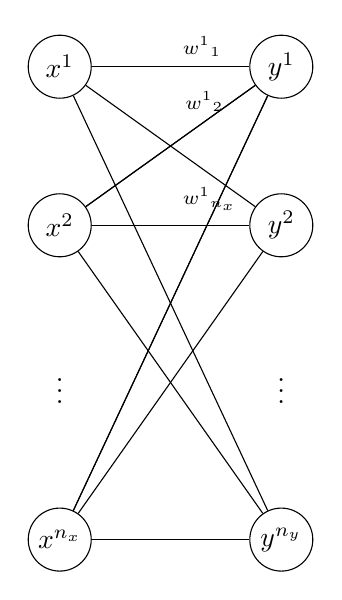
\begin{tikzpicture}[
    node distance=1.2cm and 2cm,
    varnode/.style={circle, draw, minimum size=8mm, inner sep=0pt},
    edgelabel/.style={font=\scriptsize, above, pos=0.7} % label above edge near y
]


% Input nodes
\node[varnode] (x1) {$x^1$};
\node[varnode, below=of x1] (x2) {$x^2$};
\node[below=of x2] (x3) {$\vdots$}; % no circle
\node[varnode, below=of x3] (xn) {$x^{n_x}$};

% Output nodes
\node[varnode, right=of x1] (y1) {$y^1$};
\node[varnode, below=of y1] (y2) {$y^2$};
\node[below=of y2] (y3) {$\vdots$}; % no circle
\node[varnode, below=of y3] (yn) {$y^{n_y}$};

% Edges
\foreach \i/\x in {1/x1,2/x2,n/xn}{
  \foreach \j/\y in {1/y1,2/y2,n/yn}{
    \draw (\x) -- (\y);
  }
}

% Labels only for edges into y1
\foreach \i/\x in {1/x1,2/x2,n_x/xn}{
  \draw (\x) -- (y1) node[edgelabel] {${w^{1}}_{\i}$};
}

\end{tikzpicture}
\end{center}

If we define $\vw$ as a column vector with all of the entries of $W$ in one column, we are interested in the two quantities:
$D_\vw \vy$ and $D_\vb \vy$. These will allow us to compute the gradient of the error later with respect to these inputs.

\[ \vw =\begin{bmatrix}
  {w^1}_1 \\
  {w^1}_2 \\
  \vdots \\
  {w^1}_m \\
  {w^2}_1 \\
  \vdots \\
  {w^n}_m
\end{bmatrix} \]

The benefit of using a linear combination is that it is ``simple'' to find the Jacobian matrix. 
First we introduce the \emph{Kronecker delta} ${\delta^i}_j$ to be $1$ when $i=j$ and $0$ otherwise. 
This is essential because $\del{x^i}{x^j} = {\delta^i}_j$ for independent variables. 
Note also that ${\delta^i}_\rho x^\rho = x^i$, where we are summing over repeated variables.
Then we calculate (slightly abusing matrix notation and using shorthand):

\begin{align*}  
  (D_\vw \vy) &=  \del{y^i}{{w^j}_k} \\
   &= \partial_{{w^j}_k} (y^i) \tag{shorthand for partial derivative}\\
   &= \partial_{{w^j}_k} ({w^i}_\rho x^\rho + b^i) \tag{substituting $y$ definition}\\
   &= x^\rho \partial_{{w^j}_k} ({w^i}_\rho) \tag{linearity of partial derivative}\\
   &= x^\rho {\delta^i}_j {\delta^k}_\rho \tag{independence of variables}\\
   &= x^k {\delta^i}_j \tag{summing over Kronecker delta}
\end{align*}
\begin{align*}  
  (D_\vb \vy) &=  \del{y^i}{{b^j}} \\
   &= \partial_{{b^j}} (y^i) \tag{shorthand for partial derivative}\\
   &= \partial_{{b^j}} ({w^i}_\rho x^\rho + b^i) \tag{substituting $y$ definition}\\
   &= \partial_{{b^j}} ({b^i}) \tag{linearity of partial derivative}\\
   &= {\delta^i}_j 
\end{align*}

Again, we consider $D_\vw \vy$ to be a matrix by considering $\vw$ as a vector.

It will also be useful to compute the next quantity for later.

\begin{align*}
  (D_\vx \vy) &=   \del{y^i}{{x^j}} \\
   &= \partial_{{x^j}} (y^i) \tag{shorthand for partial derivative}\\
   &= \partial_{{x^j}} ({w^i}_\rho x^\rho) \tag{substituting $y$ definition}\\
   &= {w^i}_\rho\partial_{{x^j}}(x^\rho)  \tag{linearity of partial derivative}\\
   &= {w^i}_\rho {\delta^\rho}_j \tag{independence of variables}\\
   &= {w^i}_j \tag{summing over Kronecker delta}
\end{align*}

Hence we have found the following.

\begin{proposition}\label{prop:jacobian-linear-comb}
  Define $\vy = W \vx + \vb$ for a matrix $W$ and vectors $\vx$ and $\vb$. 
  Let $\delta$ denote the \emph{Kronecker delta} ${\delta^i}_j$ to be $1$ when $i=j$ and $0$ otherwise. 
  Consider $W$ as a vector via the following construction.
  \[ \vw =\begin{bmatrix}
  {w^1}_1 \\
  {w^1}_2 \\
  \vdots \\
  {w^1}_m \\
  {w^2}_1 \\
  \vdots \\
  {w^n}_m
\end{bmatrix} \]

Then we have the following:
  \begin{enumerate}
    \item ${(D_\vw \vy)^i}_{jk} =x^k {\delta^i}_j$
    \item ${(D_\vb \vy)^i}_j = {\delta^i}_j $
    \item ${(D_\vx \vy)^i}_j = {w^i}_j $
  \end{enumerate}
Where we consider the former as a matrix by converting the lower $(jk)$ indices into a vector as we did with $W$ itself.
\end{proposition}

Let's also choose an $E = E(\vy)$ which we can compute the Jacobian matrix of ``simply''. 
Let $|| \cdot ||$ denote the Euclidean norm and define $E$ as:
\[ E(\vy; \vyh_{(i)}) = \frac{1}{2} ||\vy - \vyh_{(i)} ||^2 = \frac{1}{2} (\vy - \vyh_{(i)})^T(\vy - \vyh_{(i)}) \]

Then consider 
\begin{align*}
  (D_\vy E)_j &= \del{E}{y^j} \\
   &= \frac{1}{2} \partial_{y^j} \left((y^j)^2 - 2 y^j \widehat{y}^j - (\widehat{y}^j)^2 \right) \tag{no sum over $j$} \\
   &= \frac{1}{2} (2y^j - 2 \widehat{y}^j) \\
   &= y^j - \widehat{y}^j
  \end{align*}

Hence, carefully keeping track of indices, we find the following.

\begin{proposition} \label{prop:jacobian-square-error}
Let $|| \cdot ||$ denote the Euclidean norm and define $E$ as:
\[ E(\vy; \vyh_{(i)}) = \frac{1}{2} ||\vy - \vyh_{(i)} ||^2\]
Then 
\[ D_\vy E(\vy; \vyh) = (\vy - \vyh )^T\]
  
\end{proposition}
Therefore, we can finally compute:

\[ \nabla_\vw E = (D_\vw E)^T = (D_\vy E D_\vw \vy)^T \]

Hence. we can substitute the above formulae to conduct gradient descent Theorem \ref{th:gradient-descent-nd-mom-wind} 
and minimise $E$ with respect to $\vw$ and $\vb$. 
Unfortunately while this would work, this is completely linear, and therefore will be able to find linear solutions.

How do we introduce non-linearity? Moreover, how do we ensure that introducing non-linearity still enables us to compute the Jacobian simply?

The simplest way to introduce some non-linearity is to add a non-linear function between $y$ and $E$.

To account for this, let's introduce a (non-linear) function $\vsigma$ which takes in a vector and outputs a vector of the same length, 
and also do some relabeling and book-keeping:
\begin{align*}
  \vz &= W \vx + \vb \\
  \vy &= \vsigma (\vz)
\end{align*}

Moreover, if $\vsigma$ is defined such that it is a component-wise application of a function $\sigma$, then 

\[ {(D_\vz \vsigma)^i}_j =  \frac{d\sigma}{dz^j}\]

An important choice of $\sigma$ (that we extend component-wise to $\vsigma$) which achieves our desire is the \emph{sigmoid} function
\[ \sigma(x) = \frac{1}{1 + e^{-x}}\]

This is because the sigmoid function is non-linear, and we can write the gradient of $\sigma$ in terms of $\sigma$ itself:
 \begin{align*}
  \frac{d \sigma}{dx}(x) &= e^{-x} \frac{1}{(1 + e^{-x})^2} \\
   &= \sigma(x) \frac{e^{-x} }{1 + e^{-x}} \\
   &= \sigma(x) \frac{(1 + e^{-x} ) -1}{1 + e^{-x}} \\
   &= \sigma(x) \left(1 -\frac{1}{1 + e^{-x}} \right)\\
   &= \sigma(x) (1 - \sigma(x))
 \end{align*}

Hence, we find that 

\begin{proposition} \label{prop:jacobian-sigmoid}
If $\vsigma$ is constructed as the component-wise extension of the sigmoid function $\sigma$, 
\[ {(D_\vz \vsigma)^i}_j =  \frac{d\sigma}{dz^j} = \sigma(z^j) (1 - \sigma(z^j))\]
  
\end{proposition}

\subsubsection{Neural Networks with One Layer Formulation}

So we have the setup
\begin{align}
  \vz &= W \vx + \vb \label{eq:z-linear-comb}\\
  \vy &= \vsigma (\vz) \label{eq:y-sigma-z}\\
  E &= E(\vy; \vyh) = E(\vsigma(\vz); \vyh) \label{eq:E-vy-vyh}
\end{align}

The components of $W$ are called \emph{weights} and the components of $\vb$ are called \emph{bias}.

We can now combine the results from Theorem \ref{th:generalised-chain-rule} and 
Propositions \ref{prop:jacobian-linear-comb}, \ref{prop:jacobian-sigmoid}, and 
\ref{prop:jacobian-square-error}\footnote{The latter two are based on our choice of $\vsigma$ and $E$; we have chosen $\vsigma$ to be the sigmoid function, and $E$ to be the square error for consistency}.
 to get the main result of this section.

\begin{theorem} \label{th:nn-one-layer}
  Gradient descent formula for a simple neural network.

  Given the setup above, we have that
  \begin{align*}
\nabla_\vw E &= (D_\vsigma E D_\vz \vsigma D_\vw \vz)^T \\
\nabla_\vb E &= (D_\vsigma E D_\vz \vsigma D_\vb \vz)^T
\end{align*}

These can be fed into the gradient descent algorithm Theorem \ref{th:gradient-descent-nd-mom-wind}.
\end{theorem}

The main thing that makes the above possible to interpret as an algorithm, 
is that the results of each Jacobian above can be written in terms of the variables $\vz$, $\vy$, and $\vx$. 
Hence, given a fixed $\vx = \vxh$ and some numbers (e.g. initially randomly chosen) weights $W$ and bias $\vb$, 
we can find how our error function $E$ changes with respect to $W$ and $\vb$ with only computing Equations
\ref{eq:z-linear-comb}, \ref{eq:y-sigma-z}, and \ref{eq:E-vy-vyh}. 
Computing Equations
\ref{eq:z-linear-comb}, \ref{eq:y-sigma-z}, and \ref{eq:E-vy-vyh} 
involves feeding numbers through each in order, this is often called \emph{forward propagation}, or a \emph{forward pass}. 
Computing the gradients in Theorem \ref{th:nn-one-layer} is then often called \emph{backward propagation}.

Due to our knowledge of gradient descent, we know that this process will find a (local) minima of 
$E$ when viewed as a function of the weights and bias, $W$ and $\vb$.

This whole process is referred to as a \emph{neural network with one layer} (the ``one layer'' can be thought of as being one set of lines between $\vx$ and $\vy$):

\begin{center}
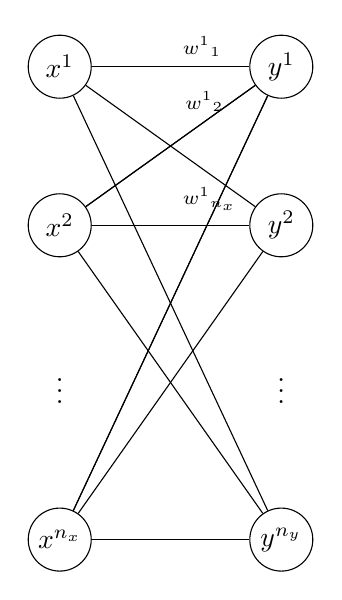
\begin{tikzpicture}[
    node distance=1.2cm and 2cm,
    varnode/.style={circle, draw, minimum size=8mm, inner sep=0pt},
    edgelabel/.style={font=\scriptsize, above, pos=0.7} % label above edge near y
]

% Input nodes
\node[varnode] (x1) {$x^1$};
\node[varnode, below=of x1] (x2) {$x^2$};
\node[below=of x2] (x3) {$\vdots$}; % no circle
\node[varnode, below=of x3] (xn) {$x^{n_x}$};

% Output nodes
\node[varnode, right=of x1] (y1) {$y^1$};
\node[varnode, below=of y1] (y2) {$y^2$};
\node[below=of y2] (y3) {$\vdots$}; % no circle
\node[varnode, below=of y3] (yn) {$y^{n_y}$};

% Edges
\foreach \i/\x in {1/x1,2/x2,n/xn}{
  \foreach \j/\y in {1/y1,2/y2,n/yn}{
    \draw (\x) -- (\y);
  }
}

% Labels only for edges into y1
\foreach \i/\x in {1/x1,2/x2,n_x/xn}{
  \draw (\x) -- (y1) node[edgelabel] {${w^{1}}_{\i}$};
}

\end{tikzpicture}
\end{center}


A limitation which needs to be addressed is with our choice of error function in Proposition \ref{prop:jacobian-square-error}. 
This function by definition only computes the error for one $\vyh$. Our setup in Section \ref{sec:goal-revisited} requires a collection of such $\vyh_{(i)}$. 
One approach is to calculate one step of gradient descent for each pair $(\vxh_{(i)}, \vyh_{(i)})$ respectively, and take the average of the new $\vx$ as the ``actual'' step.
We will instead take another approach which also removes this issue once tensors have been introduced.

\subsection{How Good is a Single Layer Neural Network?}
How well does this neural network achieve our goal in Section \ref{sec:goal-revisited}? While it is true that this will minimise the error, this might still be 
useless for complex problems if we have not encoded enough non-linearity. Considering $\vsigma$ as the component-wise sigmoid function, 
let's unravel what $\vy$ is:

\begin{align*}
  (\vy)^i &= (\vsigma(\vz))^i \\
   &= (\vsigma ( W \vx + \vb))^i \\
   &= \sigma({w^i}_jx^j + b^i) \label{summing over repeated indices}\\ 
   &= \frac{1}{1+ e^{-({w^i}_jx^j + b^i) }} \\
   &= \frac{1}{1+ e^{-{w^i}_1x^1 }e^{-{w^i}_2x^2 }\dots e^{- b^i }}
\end{align*}

This means that our non-linearity is restricted to specifically the form of (the quotient of) some multiplications. 
This is not ``very'' non-linear, and results in this neural network not being powerful enough to solve complicated 
non-linear problems.

Also notice that we can now understand why the components of $\vb$ are called bias: the denominator has the term $ e^{- b^i }$, which pushes the entire result 
towards $0$ or $1$ when $b^i$ becomes very negative or positive respectively, introducing an overall \emph{bias} towards $0$ or $1$.

\newpage
\section{Neural Networks with Hidden Layers} \label{sec:nn-hidden-layer}
As discussed in the previous section, neural networks with one layer suffer from a lack of sufficient non-linearity.

To keep aligned with our goal of simplicity of computation in Section \ref{sec:goal-revisited}, we can reuse the work 
that led to Theorem \ref{th:nn-one-layer} by inserting more iterations of applying weights and then a non-linear function $\vsigma$.
We call these intermediate layers \emph{hidden layers}. Let $L$ be a number more than $0$ called \emph{the number of layers}. 
Define a sequence of matrices $W^{(i)}$, vectors $\vz^{(i)} $, $\va^{(i)}$, and $\vb^{(i)}$, and \emph{activation functions} $\vsigma^{(i)}$ which take vectors to vectors of the same dimension, 
for $i = 1, \dots, L$ by:

\begin{equation}\label{eq:layer-forward-prop}
\begin{aligned}
  \va^{(0)} &= \vx \\ 
  \vz^{(i)} &= W^{(i)} \va^{(i-1)} + \vb^{(i)} \\
  \va^{(i)} &= \vsigma^{(i)} \left(\vz^{(i)}\right) \\
  \vy &= \va^{(L)} \\
  E &= E(\vy; \vyh)
\end{aligned}
\end{equation}

The components of $W^{(i)}$ and $\vb^{(i)}$ are called the \emph{weights and bias for layer $i$} respectively. 
Note that we are free to choose each $\va^{(i)}$ to be any dimension (size) we would like whenever $i$ is not $0$ or $L$, 
where it must have the same dimension as $\vx$ and $\vy$ respectively. 
Moreover, given a choice of dimensions of each $\va^{(i)}$ as $n_i$, the dimensions of each $W^{(i)}$ are 
determined to be $(n_{i} \times n_{i-1})$ respectively, and $b^{(i)}$ to be a vector of length $n_i$. 
Note we interpret $n_0 = n_x$ and $n_L = n_y$.
We can visualise this again in graph form as the following:

\begin{center}
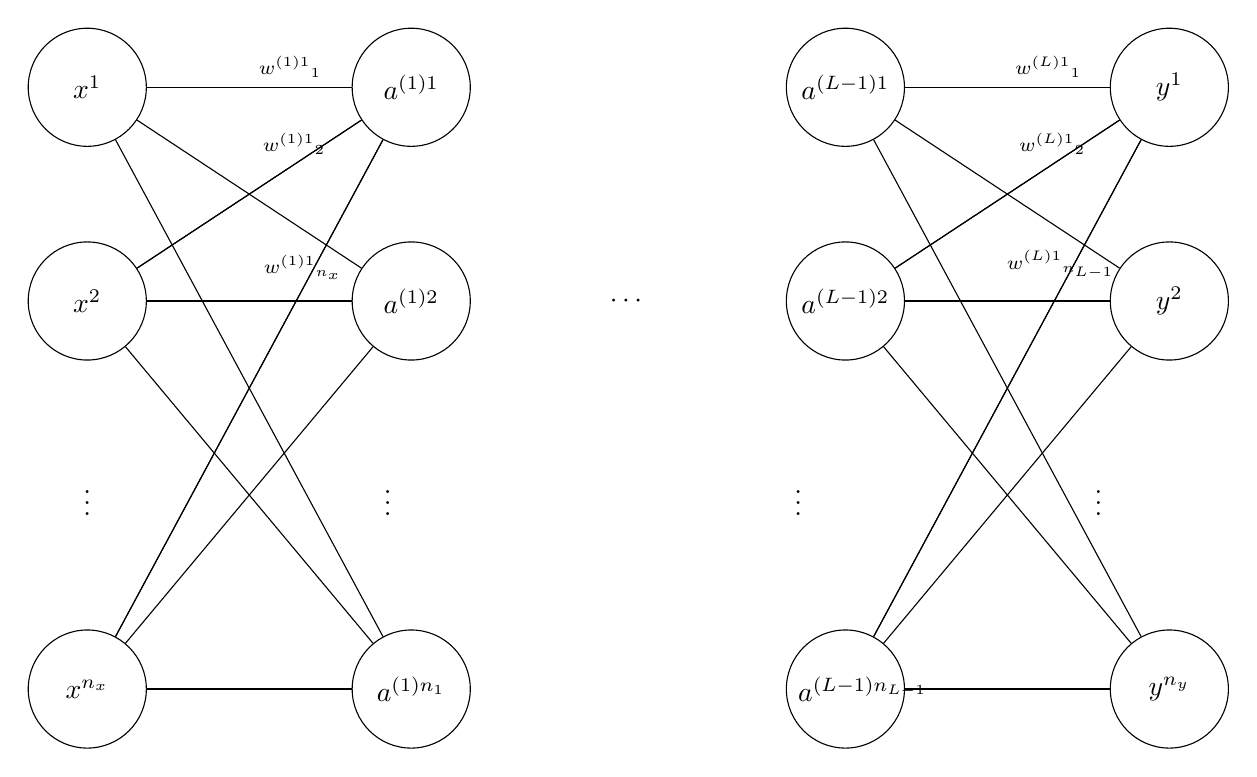
\begin{tikzpicture}[
    node distance=12mm and 26mm,
    varnode/.style={circle, draw, minimum size=15mm, inner sep=0pt, text width=12mm, align=center},
    dotnode/.style={minimum size=10mm, inner sep=0pt, text width=12mm, align=center},
    edgelabel/.style={font=\scriptsize, above, pos=0.7} % label above edge, closer to right node
]

% --- Input layer ---
\node[varnode] (x1) {$x^1$};
\node[varnode, below=of x1] (x2) {$x^2$};
\node[dotnode, below=of x2] (x3) {$\vdots$};
\node[varnode, below=of x3] (xn) {$x^{n_x}$};

% --- First hidden layer ---
\node[varnode, right=of x1] (a11) {$a^{(1)1}$};
\node[varnode, right=of x2] (a12) {$a^{(1)2}$};
\node[dotnode, right=of x3] (a13) {$\vdots$};
\node[varnode, right=of xn] (a1n) {$a^{(1)n_1}$};

% --- Last hidden layer (aligned row-by-row to the first hidden layer) ---
\node[varnode, right=40mm of a11] (aL11) {$a^{(L-1)1}$};
\node[varnode, right=40mm of a12] (aL12) {$a^{(L-1)2}$};
\node[dotnode, right=40mm of a13] (aL13) {$\vdots$};
\node[varnode, right=40mm of a1n] (aL1n) {$a^{(L-1)n_{L-1}}$};

% --- Output layer (aligned row-by-row to last hidden layer) ---
\node[varnode, right=of aL11] (y1) {$y^1$};
\node[varnode, right=of aL12] (y2) {$y^2$};
\node[dotnode, right=of aL13] (y3) {$\vdots$};
\node[varnode, right=of aL1n] (yn) {$y^{n_y}$};

% --- Decorative horizontal dots between hidden layers (placed after nodes so it doesn't affect alignment) ---
\node[dotnode] at ($(a12)!0.5!(aL12)$) {$\cdots$};

% --- Edges: x -> a^(1) (fully connected) ---
\foreach \i/\x in {1/x1,2/x2,n/xn}{
  \foreach \j/\y in {1/a11,2/a12,n/a1n}{
    \draw (\x) -- (\y);
  }
}
% Labels only for edges into a^(1)1
\foreach \i/\x in {1/x1,2/x2,n_x/xn}{
  \draw (\x) -- (a11) node[edgelabel] {${w^{(1)1}}_{\i}$};
}

% --- Edges: a^(L-1) -> y (fully connected) ---
\foreach \i/\x in {1/aL11,2/aL12,n/aL1n}{
  \foreach \j/\y in {1/y1,2/y2,n/yn}{
    \draw (\x) -- (\y);
  }
}
% Labels only for edges into y1
\foreach \i/\x in {1/aL11,2/aL12,n_{L-1}/aL1n}{
  \draw (\x) -- (y1) node[edgelabel] {${w^{(L)1}}_{\i}$};
}

\end{tikzpicture}
\end{center}

Now we have many parameters that we wish to vary to minimise our error function $E$. 
We can repeatedly apply the Chain Rule Theorem \ref{th:generalised-chain-rule} to compute 
each quantity we desire by considering $E$ as a function of the weights and bias, unraveling the sequence in 
Sequence \ref{eq:layer-forward-prop}. 
Moreover, we can collapse each matrix $W^{(i)}$ into a vector $\vw^{(i)}$ as in Proposition \ref{prop:jacobian-linear-comb}.

For example, temporarily suppressing $\vyh$ for clarity, we may unravel Sequence \ref{eq:layer-forward-prop} until we find $\vw$ or $\vb$:

\begin{align*}
  E = E(\vy) &= E\left(\va^{(L)}\right) \\
  E &= E\left(\vsigma^{(L)}\left(\vz^{(L)}\right)\right) \\
  E &= E\left(\vsigma^{(L)}\left(\vz^{(L)} \left( \vw^{(L)} \right)\right)\right) \tag{found a $\vw$}\\
  E &= E\left(\vsigma^{(L)}\left(\vz^{(L)} \left( \vb^{(L)} \right)\right)\right) \tag{found a $\vb$}\\
  E &= E\left(\vsigma^{(L)}\left(\vz^{(L)} \left( \textcolor{red}{\va^{(L-1)} }\right)\right)\right) \\
  E &= E\left(\vsigma^{(L)}\left(\vz^{(L)} \left( \textcolor{red}{\vsigma^{(L-1)} \left( \vz^{(L-1)} \right)} \right)\right)\right) \\
  E &= E\left(\vsigma^{(L)}\left(\vz^{(L)} \left( \textcolor{red}{\vsigma^{(L-1)} \left( \vz^{(L-1)} \left( \vw^{(L-1)} \right) \right)} \right)\right)\right) \tag{found a $\vw$}\\
  E &= E\left(\vsigma^{(L)}\left(\vz^{(L)} \left( \textcolor{red}{\vsigma^{(L-1)} \left( \vz^{(L-1)} \left( \vb^{(L-1)} \right) \right)} \right)\right)\right) \tag{found a $\vb$}\\
  E &= E\left(\vsigma^{(L)}\left(\vz^{(L)} \left( \vsigma^{(L-1)} \left( \vz^{(L-1)} \left( \textcolor{red}{\va^{(L-2)}} \right) \right) \right)\right)\right) \\
   &\vdots
\end{align*}

Due to this unraveling process, it is also helpful to compute the gradients ``backwards'' via repeatedly applying the Chain Rule Theorem \ref{th:generalised-chain-rule}, utilising the lines above when $\vw$ and $\vb$ appear, also recalling Proposition \ref{prop:gradient-as-jacobian}:

\begin{align*}
  \nabla_{\vw^{(L)}}E = \left(D_{\vw^{(L)}}E\right)^T &= \left(D_{\vsigma^{(L)}}E D_{\vz^{(L)}}\vsigma^{(L)} D_{\vw^{(L)}}\vz^{(L)}\right)^T \\
  \nabla_{\vb^{(L)}}E = \left(D_{\vb^{(L)}}E\right)^T &= \left(D_{\vsigma^{(L)}}E D_{\vz^{(L)}}\vsigma^{(L)} D_{\vb^{(L)}}\vz^{(L)}\right)^T \\
  \nabla_{\vw^{(L-1)}}E = \left(D_{\vw^{(L-1)}}E\right)^T &= \left(D_{\vsigma^{(L)}}E D_{\vz^{(L)}}\vsigma^{(L)} 
  \textcolor{red}{D_{\vsigma^{(L-1)}}\vz^{(L)} D_{\vz^{(L-1)}} \vsigma^{(L-1)}}
  D_{\vw^{(L-1)}}\vz^{(L-1)}\right)^T \\
  \nabla_{\vb^{(L-1)}}E = \left(D_{\vb^{(L-1)}}E\right)^T &= \left(D_{\vsigma^{(L)}}E D_{\vz^{(L)}}\vsigma^{(L)} 
  \textcolor{red}{D_{\vsigma^{(L-1)}}\vz^{(L)} D_{\vz^{(L-1)}} \vsigma^{(L-1)}} 
  D_{\vb^{(L-1)}}\vz^{(L-1)}\right)^T  \\
   &\vdots
\end{align*}

Continuing unraveling down to layer $1$, we derive the following result.

\begin{theorem} \label{th:nn-L-layer}
  Gradient descent formula for a neural network with $L$ layers.

  Let $i$ be a number more than $0$ but less than $L$. Given the setup above, we have that:
\begin{align*}
  \nabla_{\vw^{(L)}}E = \left(D_{\vw^{(L)}}E\right)^T &= \left(D_{\vsigma^{(L)}}E D_{\vz^{(L)}}\vsigma^{(L)} D_{\vw^{(L)}}\vz^{(L)}\right)^T \\
  \nabla_{\vb^{(L)}}E = \left(D_{\vb^{(L)}}E\right)^T &= \left(D_{\vsigma^{(L)}}E D_{\vz^{(L)}}\vsigma^{(L)} D_{\vb^{(L)}}\vz^{(L)}\right)^T \\
  \nabla_{\vw^{(i)}}E = \left(D_{\vw^{(i)}}E\right)^T &= \left(D_{\vsigma^{(L)}}E D_{\vz^{(L)}}\vsigma^{(L)} 
  \textcolor{red}{
    \left(\prod_{j = L-1}^{i}D_{\vsigma^{(j)}}\vz^{(j+1)} D_{\vz^{(j)}} \vsigma^{(j)}\right)
    }
  D_{\vw^{(i)}}\vz^{(i)}\right)^T \\
  \nabla_{\vb^{(i)}}E = \left(D_{\vb^{(i)}}E\right)^T &= \left(D_{\vsigma^{(L)}}E D_{\vz^{(L)}}\vsigma^{(L)} 
  \textcolor{red}{
    \left(\prod_{j = L-1}^{i}D_{\vsigma^{(j)}}\vz^{(j+1)} D_{\vz^{(j)}} \vsigma^{(j)}\right)
    } 
  D_{\vb^{(i)}}\vz^{(i)}\right)^T 
\end{align*} 
  Where the terms highlighted in red denote a descending right product of terms:
  \[
  \prod_{j=L-1}^{i} A^{(i)} = A^{(L-1)}A^{(L-2)}\dots A^{(i+1)} A^{(i)}
  \]


  These can be fed into the gradient descent algorithm Theorem \ref{th:gradient-descent-nd-mom-wind}.
\end{theorem}

The main thing that makes the above possible to interpret as an algorithm such as in Theorem \ref{th:nn-one-layer}, 
is that the results of each Jacobian above can be written in terms of the variables $\vz^{(i)}$ and $\va^{(i)}$. 
This is achieved by substituting the relevant vectors and matrices into 
Propositions \ref{prop:jacobian-linear-comb}, \ref{prop:jacobian-sigmoid}, and \ref{prop:jacobian-square-error}.\footnote{The latter two are based on our choice of $\vsigma^{(i)}$ and $E$; we have chosen each $\vsigma^{(i)}$ to be the sigmoid function, and $E$ to be the square error for consistency}

For example, 

\begin{align*}
  \vz^{(j+1)} &= W^{(j+1)} \vsigma^{(j)} \left(\vz^{(j)}\right)  + \vb^{(j+1)} \\
  D_{\vsigma^{(j)}}\vz^{(j+1)} &= W^{(j+1)} \tag{Equation 3 Proposition \ref{prop:jacobian-linear-comb}}
\end{align*}

Hence, given a fixed $\vx = \vxh$ and some numbers (e.g. initially randomly chosen) weights $W^{(i)}$ and bias $\vb^{(i)}$ for each layer, 
we can find how our error function $E$ changes with respect to a specific layer's $W^{(i)}$ or $\vb^{(i)}$ with only computing the equations in Sequence
\ref{eq:layer-forward-prop}. 

Computing the equations in Sequence
\ref{eq:layer-forward-prop}
involves feeding numbers through each in order, this is often called \emph{forward propagation}. 
Computing the gradients in Theorem \ref{th:nn-one-layer} is then often called 
\emph{backward propagation} due to the amount of repeated Jacobians as you go ``backwards'' in $i$ values
-- these do not need to be recomputed each time, which saves a lot of computational expense over computing each Jacobian each time.

Due to our knowledge of gradient descent, we know that this process will find a (local) minima of 
$E$ when viewed as a function of the weights and bias of each layer, $W^{(i)}$ and $\vb^{(i)}$.

This whole process is referred to as a \emph{neural network with $L$ layers} (the ``$L$ layers'' can be thought of as being $L$ sets of lines between $\va^{(i-1)}$ and $\va^{(i)}$ in our diagram).

A limitation which needs to again be addressed is with our choice of error function in Proposition \ref{prop:jacobian-square-error}. 
This function by definition only computes the error for one $\vyh$. Our setup in Section \ref{sec:goal-revisited} requires a collection of such $\vyh_{(i)}$. 
One approach is to calculate one step of gradient descent for each pair $(\vxh_{(i)}, \vyh_{(i)})$ respectively, and take the average of the new $\vx$ as the ``actual'' step.
We will take another approach by incorporating the entire training dataset into our neural network algorithm via tensors.
\newpage
\section{Tensors} \label{sec:tensors}

We would like to deal with many samples of training data $\vxh$ simultaneously. 
To do so, we first need to develop a framework where we can generalise gradient descent 
Theorem \ref{th:gradient-descent-nd-mom-wind} and the chain rule Thereom \ref{th:generalised-chain-rule} 
to higher dimensional objects. One can view the motivation behind doing so in the first equation of 
Proposition \ref{prop:jacobian-linear-comb} -- we have no sensible way of interpreting the three indices 
without collapsing them into less indices as a result of an awkward reshaping process.

A tensor is an \emph{arbitrary (finite) dimensional array of numbers}.\footnote{This is a small simplification of the usual notion of tensors, but it is sufficient for our purposes.}
We say $T$ is a \emph{tensor of type $(r,s)$} or an \emph{$(r,s)$ tensor} for short if it has $r$ superscript indices and $s$ subscript indices:

\[ {T^{\mu_1 \mu_2 \dots \mu_r}}_{\nu_1 \nu_2 \dots \nu_s}\]

In this way, a matrix $A$ is a tensor of type $(1,1)$; it has two indices ${A^i}_j$. We allow $r$ or $s$ to be zero to represent no indices. 
In this way, a column vector $\vx$ is a tensor of type $(1,0)$; it has one upper index $x^i$. 
A row vector $\vx^T$ will be considered a tensor of type $(0,1)$; it has one lower index $x_j$. 
A number $\alpha$ (often called a scalar) is a tensor of type $(0,0)$; it has no indices.

Due to convenience, we will ignore the range of values each index can take. 
We are allowing each index to take on a range of values independently.
If required, we could refer to an $(r,s)$ tensor as being of shape $(n_{\mu_1}, \dots, n_{\mu_r}, m_{\nu_1}, \dots, m_{\nu_s})$ to specify the range that each index can vary over.
In this way, an $(n\times m)$ matrix is a $(1,1)$ tensor of shape $(n,m)$, a column vector of dimension $n$ is a $(1,0)$ tensor of shape $(n)$. 
This is aligned to how the Python package NumPy defines tensors in terms of shape\footnote{NumPy does not distinguish between upper or lower indices. One reason we have been so pedantic with horizontal spacing is so that we can more simply code the order of tensor indices by reading them left to right.}.

It is time to return to the Einstein Summation convention which we have used sporadically. 
Let's consider two tensors, an $(r,s)$ tensor T and a $(p,q)$ tensor S. 
If a lower/upper index of T is denoted with the same letter as an upper/lower index of S respectively, 
and the range of values the two indices can take are same and equal to $n_i$ (the corresponding shape for the respective tensors are the same for that index), 
then we sum over the full range of that repeated index.
\begin{align*}
{T^{\mu_1 \dots \textcolor{red}{i} \dots \mu_r}}_{\nu_1 \dots \nu_s} &{S^{\rho_1 \dots \rho_p}}_{\sigma_1 \dots \textcolor{red}{i} \dots \sigma_q} \\
 &= {T^{\mu_1 \dots \textcolor{red}{1} \dots \mu_r}}_{\nu_1 \dots \nu_s} {S^{\rho_1 \dots \rho_p}}_{\sigma_1 \dots \textcolor{red}{1} \dots \sigma_q} \\
 &+ {T^{\mu_1 \dots \textcolor{red}{2} \dots \mu_r}}_{\nu_1 \dots \nu_s} {S^{\rho_1 \dots \rho_p}}_{\sigma_1 \dots \textcolor{red}{2} \dots \sigma_q} \\
 &+ \dots \\
 &+ {T^{\mu_1 \dots \textcolor{red}{n_i} \dots \mu_r}}_{\nu_1 \dots \nu_s} {S^{\rho_1 \dots \rho_p}}_{\sigma_1 \dots \textcolor{red}{n_i} \dots \sigma_q}
\end{align*}

Here we can see explicitly why we required that the range of values that the summed indices can take to be equal; we do not want any leftover indices after the sum.
In this way, we can consider the resulting tensor to be a tensor of type $(r+p-1,s+q-1)$, since we have explicitly summed over one upper and one lower index.
This process is usually referred to as \emph{contracting indices}, and it is a functionality included in the Python library NumPy via the function \emph{einsum}.

Note that we can contract multiple indices by contracting them one at a time.

We can now interpret matrix multiplication of an $(n \times m)$ matrix $A$ and an $(m \times k)$ matrix $B$ as contracting a
$(1,1)$ tensor $A$ of shape $(n,\textcolor{red}{m})$ and a $(1,1)$ tensor $B$ of shape $(\textcolor{red}{m},k)$:

\[ {(AB)^i}_j = {A^i}_{\textcolor{red}{k}} {B^{\textcolor{red}{k}}}_j\]

The output $AB$ is itself a $(1,1)$ tensor of shape $(n,k)$.

\subsection{Tensor Calculus: the Tensor Jacobian and Gradient}
We wish to work our way to some notion of gradient descent Theorem \ref{th:gradient-descent-nd-mom-wind}, but for tensors. 
We will approach this by generalising the Jacobian Definition \ref{def:jacobian}, generalising the chain rule Theorem \ref{th:generalised-chain-rule} to tensors, 
and taking inspiration from Proposition \ref{prop:gradient-as-jacobian}.

For this section, let $T$ be an $(r,s)$ tensor, $S$ be a $(p,q)$ tensor, and $R$ be an $(m,n)$ tensor. Moreover, let 
$T = T(S)$ and $S = S(R)$ be sufficiently smooth functions of the components of their respective argument tensor.

\begin{definition} \label{def:tensor-jacobian}
  The Jacobian Tensor

  Let $T$ and $S$ be as above. Define the \emph{Jacobian Tensor of $T$} denoted $D_S T$ to be an $(r+q,s+p)$ tensor defined by the following:

  \[ {(D_S T)^{\mu_1 \dots \mu_r \sigma_1 \dots \sigma_q }}_{\nu_1 \dots \nu_s \rho_1 \dots \rho_p} = 
  \del{{T^{\mu_1 \dots \mu_r  }}_{\nu_1 \dots \nu_s}}
  {{S^{\rho_1 \dots \rho_p}}_{\sigma_1 \dots \sigma_q }}\]

  Warning: pay attention to the ordering of the indices.
\end{definition}

Notice that when $T$ and $S$ are (column) vectors or scalars, we recover the Jacobian defined in Definition \ref{def:jacobian}.

We will now consider two Jacobian tensors $D_S T$ and $D_R S$. Observe the following contraction of indices:

\begin{align*}
  {(D_S T)^{\mu_1 \dots \mu_r \textcolor{red}{\sigma_1 \dots \sigma_q }}}_{\nu_1 \dots \nu_s \textcolor{blue}{\rho_1 \dots \rho_p}} 
  &{(D_R S)^{\textcolor{blue}{\rho_1 \dots \rho_p} \delta_1 \dots \delta_n }}_{ \textcolor{red}{\sigma_1 \dots \sigma_q } \kappa_1 \dots \kappa_m} \\
  &=   \del{{T^{\mu_1 \dots \mu_r  }}_{\nu_1 \dots \nu_s}}
  {{S^{\textcolor{blue}{\rho_1 \dots \rho_p}}}_{\textcolor{red}{\sigma_1 \dots \sigma_q }  }}   \del{{S^{\textcolor{blue}{\rho_1 \dots \rho_p}}}_{\textcolor{red}{\sigma_1 \dots \sigma_q }  }}
  {{R^{\kappa_1 \dots \kappa_m}}_{\delta_1 \dots \delta_n  }} \\
  &=  \del{{T^{\mu_1 \dots \mu_r  }}_{\nu_1 \dots \nu_s}}
  {{R^{\kappa_1 \dots \kappa_m}}_{\delta_1 \dots \delta_n  }} \tag{repeated application of Theorem \ref{def:chain-rule-total-derivative}} \\
  &= {(D_R T)^{\mu_1 \dots \mu_r  \delta_1 \dots \delta_n }}_{\nu_1 \dots \nu_s \kappa_1 \dots \kappa_m}
\end{align*}

Hence we have found a way of generalising the chain rule Theorem \ref{th:generalised-chain-rule} to tensors.

\begin{theorem} \label{th:tensor-chain-rule}
  The Chain Rule for Tensor Jacobians

  Let $T$ be an $(r,s)$ tensor, $S$ be a $(p,q)$ tensor, and $R$ be an $(m,n)$ tensor. Moreover, let 
  $T = T(S)$ and $S = S(R)$ be sufficiently smooth functions of the components of their respective argument tensor.

  Define a multiplication on the Jacobian Tensor $D_T S$ of type $(r+q,s+p)$ and the Jacobian Tensor $D_S T$ of type $(p+n,q+m)$ by forming 
  a $(r+n,s+m)$ tensor via the following:

  \[ {(D_S T D_R S)^{\mu_1 \dots \mu_r  \delta_1 \dots \delta_n }}_{\nu_1 \dots \nu_s \kappa_1 \dots \kappa_m} = 
  {(D_S T)^{\mu_1 \dots \mu_r \textcolor{red}{\sigma_1 \dots \sigma_q }}}_{\nu_1 \dots \nu_s \textcolor{blue}{\rho_1 \dots \rho_p}} 
  {(D_R S)^{\textcolor{blue}{\rho_1 \dots \rho_p} \delta_1 \dots \delta_n }}_{ \textcolor{red}{\sigma_1 \dots \sigma_q } \kappa_1 \dots \kappa_m} \]

  Then we have the following result:

  \[ D_S T D_R S = D_R T\]
\end{theorem}

Inspired by Proposition \ref{prop:gradient-as-jacobian}, we wish to define the gradient of a function that takes in tensors.
First we need to define the tensor transpose.
\begin{definition} \label{def:transpose-tensor}
  Let $S$ be an $(r,s)$ tensor, then define an $(s,r)$ tensor denoted $S^T$ called \emph{the transpose of $S$} by the following:
  \[{(S^T)^{\nu_1 \dots \nu_s}}_{\mu_1 \dots \mu_r} = {S^{\mu_1 \dots \mu_r}}_{\nu_1 \dots \nu_s}\]
  
\end{definition}
Note that when $S$ is a matrix or a vector, the transpose is equivalent to our existing notion of transposing.

\begin{definition} \label{def:gradient-as-tensor-jacobian}
  Gradient of a Tensor Function

  Given a $(0,0)$ tensor $f$ and an $(r,s)$ tensor $T$ such that $f = f(T)$ is a sufficiently smooth function of the components of $T$,
  define the \emph{gradient of $f$ with respect to $T$} denoted $\nabla_T f$ by the following:
  \[ \nabla_T f = (D_T f)^T\]

  Here, the superscript $T$ denotes transposing.
\end{definition}

Note that when $T$ is a (column) vector, we have that the gradient in Definition \ref{def:gradient-as-tensor-jacobian} is equivalent to 
the gradient in Definition \ref{prop:gradient-as-jacobian}.

Now we are ready to define gradient descent for a tensor function $E$, generalising Theorem \ref{th:gradient-descent-nd-mom-wind}. 
Note that if $\alpha$ is a constant, and $T$, $S$ are two tensors of the same type, we can define $\alpha T$ to be component-wise multiplication 
by $\alpha$, and $T + S$ to be respective component-wise addition, resulting in another tensor of the same type. This is in the same spirit with how 
we defined the same notions for matrices and vectors in previous sections.

\begin{theorem}
  Gradient Descent of a Tensor Function with Momentum and Wind (Noise)
  
  Let $T$ be an $(r,s)$ tensor and let $E = E(T)$ be a non-negative $(0,0)$ tensor which is a function of $T$ in a sufficiently smooth way.
  Let $\alpha, \; \beta \in (0,1]$ be numbers between zero and one called the learning rate and the momentum parameter respectively. 
  Let $\Gamma$ be an $(r,s)$ tensor of random numbers all centered around 0, and let 
  $g: \N \rightarrow \R; \; g: n \mapsto g(n)$ be a real-valued function of 
  the current iteration called the noise parameter.
  Let $T_n$ be a sequence of $(r,s)$ tensors defined by the iterative process:
  \[ T_{n+1} = T_n - \alpha \nabla_T E \big|_{T = T_n} - \beta (T_{n} - T_{n-1}) + g(n)\Gamma \]

  Where the bar denotes evaluating the gradient at each point $\vx_n$ respectively. Then, for an appropriate choice of $\alpha, \; \beta, \; g$,
  we have that $T_n$ approaches a local minimum of $E$ as $n$ increases.

  The parameters $\alpha, \; \beta, \; g$ are referred to as hyperparameters.
\end{theorem}

The simplest way to prove the above result is by reshaping each tensor into long vectors, where it becomes equivalent to Theorem \ref{th:gradient-descent-nd-mom-wind}. 
The rest of the work is then carefully writing that reshaping map and chasing tensor types. 
In this way, it is also clear that the result recreates Theorem \ref{th:gradient-descent-nd-mom-wind} when $T$ is a (column) vector.
\newpage
\section{Neural Networks with Hidden Layers via Tensor Calculus}

Now that we have a sufficient framework for tensors developed in Section \ref{sec:tensors}, we can tackle the question of 
incorporating all of our training data at once in our formulation of neural networks with hidden layers in Section \ref{sec:nn-hidden-layer}.

Our sequence in Sequence \ref{eq:layer-forward-prop} only inputs a single $\vx$, whereas our goal in Section \ref{sec:goal-revisited} requires us 
to create a set of $m$ input-output pairs $(\vxh_{(j)},\vyh_{(j)})$.

Let's define an $(n_x \times m)$ matrix $\Xh$ and an $(n_y \times m)$ matrix $\Yh$ by having the $j$th column be 
$\vx_{(j)}$ and $\vy_{(j)}$ respectively:

\begin{align*}
\Xh^i_{\phantom{i}j} &= {\vx_{(j)}}^i \\ \Yh^i_{\phantom{i}j} &= {\vy_{(j)}}^i 
\end{align*} 

We store each training example as a column. Consider a matrix $W$. Then it follows that 
 \[ {(W \Xh)^i}_j = {W^i}_k {\vx_{(j)}}^k\]

Hence, the $j$th column of $W \Xh$ is equal to $W \vxh_{(j)}$.

\[ W \Xh = \begin{bmatrix}
  \uparrow &  & \uparrow \\
  W\vxh_{(1)} & \dots & W\vxh_{(m)} \\
  \downarrow & & \downarrow
\end{bmatrix}\]

Hence, we can interpret this multiplication $W \Xh$ as doing an individual multiplication of $W \vxh$ for each $\vxh$. 
To incorporate our notion of bias, we must define a matrix $B$ such that each column is $m$ repeats of the same vector $\vb$, 
i.e. $ {B^i}_j = b^i $. 
Then 

\[W \Xh + B = \begin{bmatrix}
  \uparrow &  & \uparrow \\
  W\vxh_{(1)} + \vb & \dots & W\vxh_{(m)} + \vb\\
  \downarrow & & \downarrow
\end{bmatrix}\]


This allows us to update our algorithm in Section \ref{sec:nn-hidden-layer}. 

To keep aligned with our goal of simplicity of computation in Section \ref{sec:goal-revisited}, we can reuse the work 
that led to Theorem \ref{th:nn-L-layer} by inserting matrices when applying weights and then a non-linear function $\vsigma$.
We still call intermediate layers \emph{hidden layers}. Let $L$ be a number more than $0$ called \emph{the number of layers}. 
Define a sequence of matrices $W^{(i)}$, $Z^{(i)} $, $A^{(i)}$, (column) vectors $\vb^{(i)}$ which we extend to matrices $B^{(i)}$ by having each column be $\vb^{(i)}$, and \emph{activation functions} $\vsigma^{(i)}$ which take matrices to matrices of the same dimension, 
for $i = 1, \dots, L$ by:

\begin{equation}\label{eq:matrix-layer-forward-prop}
\begin{aligned}
  A^{(0)} &= X \\ 
  Z^{(i)} &= W^{(i)} A^{(i-1)} + B^{(i)} \\
  A^{(i)} &= \vsigma^{(i)} \left(Z^{(i)}\right) \\
  Y &= A^{(L)} \\
  E &= E(Y; \Yh)
\end{aligned}
\end{equation}

Where $E$ is a an error function of $Y$ using $\Yh$ as a fixed goal. The components of $W^{(i)}$ and $\vb^{(i)}$ are called the \emph{weights and bias for layer $i$} respectively. 
Note that we are free to choose each $A^{(i)}$ to have as many rows as we would like whenever $i$ is not $0$ or $L$, 
where it must have the same number of rows as $X$ and $Y$ respectively. 
The number of columns of $A^{(i)}$ is always $m$, the number of samples.
Moreover, given a choice of number of rows for each $A^{(i)}$ as $n_i$, the dimensions of each $W^{(i)}$ are 
determined to be $(n_{i} \times n_{i-1})$ respectively, and $\vb^{(i)}$ to be a (column) vector of length $n_i$, making the $B^{(i)}$ into $(n_i \times m)$ matrices respectively. 
Note we interpret $n_0 = n_x$ and $n_L = n_y$.

We then wish to find the global minima of $E(W^{(1)},\vb^{(1)}, \dots, W^{(L)}, \vb^{(L)}; \vx) $, considering $\vx$ fixed.

Due to the results and notation we have developed in Section \ref{sec:tensors}, we can follow an identical procedure to that which we conducted
leading up to the main result Theorem \ref{th:nn-L-layer}.


\begin{theorem} \label{th:tensor-nn-L-layer}
  Gradient descent formula for a neural network with $L$ layers, using tensor calculus.

  Let $i$ be a number more than $0$ but less than $L$. Given the setup above, we have that:
\begin{align*}
  \nabla_{W^{(L)}}E = \left(D_{W^{(L)}}E\right)^T &= \left(D_{\vsigma^{(L)}}E D_{Z^{(L)}}\vsigma^{(L)} D_{W^{(L)}}Z^{(L)}\right)^T \\
  \nabla_{\vb^{(L)}}E = \left(D_{\vb^{(L)}}E\right)^T &= \left(D_{\vsigma^{(L)}}E D_{Z^{(L)}}\vsigma^{(L)} D_{\vb^{(L)}}Z^{(L)}\right)^T \\
  \nabla_{W^{(i)}}E = \left(D_{W^{(i)}}E\right)^T &= \left(D_{\vsigma^{(L)}}E D_{Z^{(L)}}\vsigma^{(L)} 
  \textcolor{red}{
    \left(\prod_{j = L-1}^{i}D_{\vsigma^{(j)}}Z^{(j+1)} D_{Z^{(j)}} \vsigma^{(j)}\right)
    }
  D_{W^{(i)}}Z^{(i)}\right)^T \\
  \nabla_{\vb^{(i)}}E = \left(D_{\vb^{(i)}}E\right)^T &= \left(D_{\vsigma^{(L)}}E D_{Z^{(L)}}\vsigma^{(L)} 
  \textcolor{red}{
    \left(\prod_{j = L-1}^{i}D_{\vsigma^{(j)}}Z^{(j+1)} D_{Z^{(j)}} \vsigma^{(j)}\right)
    } 
  D_{\vb^{(i)}}Z^{(i)}\right)^T 
\end{align*} 
  Where the terms highlighted in red denote a descending right tensor product of tensor jacobian terms, as defined in Section \ref{sec:tensors}:
  \[
  \prod_{j=L-1}^{i} D_{A^{(i-1)}}A^{(i)} = D_{A^{(L-2)}}A^{(L-1)}D_{A^{(L-3)}}A^{(L-2)}\dots D_{A^{(i)}}A^{(i+1)} D_{A^{(i-1)}}A^{(i)}
  \]


  These can be fed into the gradient descent algorithm Theorem \ref{th:gradient-descent-nd-mom-wind}.
\end{theorem}

Now, all that is left is to calculate the relevant tensor Jacobians\footnote{This section will be done in less detail due to the bulk of the work being very similar to that in previous sections, namely Section \ref{sec:goal-revisited} and Section \ref{sec:nn-hidden-layer}.} to consider the above as an algorithm.

\begin{proposition} \label{prop:nn-tensor-DZ}
  Let $Z$, $W$, $A$, $B$, $\vb$ be as in the setup above, i.e.
  \[ Z = WA + B \]
  Then
  \begin{enumerate}
    \item \[ {(D_WZ)^{il}}_{jk} = {A^l}_j {\delta^i}_k\]
    \item \[ {(D_AZ)^{il}}_{jk} = {W^i}_k {\delta^l}_j\]
    \item \[ {(D_{\vb}Z)^{i}}_{jk} = {\delta^i}_k\]
  \end{enumerate}
  Note that the derivative is independent of $j$ since each column of $B$ is identical.
\end{proposition}
\begin{proof}

  Firstly write 
  \[ {Z^i}_j = {W^i}_m{A^m}_j + {B^i}_j = {W^i}_m{A^m}_j + \vb^i\]

  Then continue:

  \begin{enumerate}
    \item ${(D_WZ)^{il}}_{jk}$
    \begin{align*}
      {(D_WZ)^{il}}_{jk} &= \del{{Z^i}_j}{{W^k}_l} \\
       &= \partial_{{W^k}_l}({W^i}_m{A^m}_j) \\
       &= {A^m}_j\partial_{{W^k}_l}({W^i}_m) \\
       &= {A^m}_j {\delta^i}_k{\delta^l}_m \\
       &= {A^l}_j {\delta^i}_k
    \end{align*}
    \item ${(D_AZ)^{il}}_{jk} $
    \begin{align*}
      {(D_AZ)^{il}}_{jk} &= \del{{Z^i}_j}{{A^k}_l} \\
       &= \partial_{{A^k}_l}({W^i}_m{A^m}_j) \\
       &= {W^i}_m\partial_{{A^k}_l}({A^m}_j) \\
       &= {W^i}_m {\delta^m}_k{\delta^l}_j \\
       &= {W^i}_k {\delta^l}_j
    \end{align*}
    \item ${(D_\vb Z)^{i}}_{jk}$
    \begin{align*}
      {(D_{\vb} Z)^{i}}_{jk} &= \del{{Z^i}_j}{\vb^k} \\
       &= \partial_{{\vb^k}}(\vb^i) \\
       &= {\delta^i}_k
    \end{align*}
  \end{enumerate}
\end{proof}

\begin{proposition}
  Let $Z$ be as above, and let $\vsigma$ be the component-wise extension of a one-variable activation function $\sigma$, i.e. 
  \[ {(\vsigma(Z))^i}_j = \sigma({Z^i}_j)\]
  Then 
  \[ {(D_Z \vsigma )^{il}}_{jk} = {\delta^i}_k {\delta^l}_j \sigma'\]
\end{proposition}
\begin{proof}
  We plug in at a point ${Z^i}_j$ denoted with a vertical bar and use the chain rule:
  \begin{align*}
    \left.{(D_Z \vsigma )^{il}}_{jk}\right\vert_{{Z^i}_j} &= \left.\del{\sigma}{{Z^k}_l} \right\vert_{{Z^i}_j}\\
     &= \del{\sigma({Z^i}_j)}{{Z^k}_l}\\
     &= \left.\sigma'\right\vert_{{Z^i}_j} \partial_{{Z^k}_l}{Z^i}_j \\
     &= \left.{\delta^i}_k {\delta^l}_j \sigma' \right\vert_{{Z^i}_j}
  \end{align*}
  This holds for all ${Z^i}_j$ and thus completes the proof.
\end{proof}

In the case of the sigmoid function, we can reuse our work in Proposition \ref{prop:jacobian-sigmoid} to find the following.
\begin{corollary} \label{prop:nn-tensor-DS}
  If $\vsigma$ is the component-wise extension of the sigmoid function, then 
  \[\left. {(D_Z \vsigma )^{il}}_{jk}\right\vert_{{Z^i}_j} = {\delta^i}_j {\delta^l}_j (\sigma({Z^i}_j)(1- \sigma({Z^i}_j)))\]
  \qed
\end{corollary}

Other activation functions are commonly used, such as the softmax function, ReLU, tanh, or even just the identity function (i.e. do nothing). These each have different purposes and strengths, and the interested reader should continue by looking into the differences.

The process above for the sigmoid function can then be repeated on e.g. the column-wise or component-wise extension of these functions to compute the tensor Jacobian.

A sketch is given for the softmax function below.\footnote{Here we start to use explicit summing notation using $\sum$ where it would be too cumbersome to use Einstein summation convention.}
\begin{example}
  Let $\vsigma_s$ be the column-wise extension of the softmax function $\sigma_s$ to matrices. I.e. if 
  \[ (\sigma_s(\vz))^i =  \frac{e^{\vz^i}}{\sum_k e^{\vz^k}}\]
  And considering $Z$ as a sequence of column vectors ${Z^i}_j = {\vz_{(j)}}^i$,
  \[ {\vsigma_s (Z)^i}_j = (\sigma_s (\vz_{(j)}))^i\]
  Then 
  \[ \left. {(D_Z \vsigma)^{il}}_{jk}\right\vert_{{Z^i}_j} = {\delta^l}_j {\vsigma_s(Z)^i}_l({\delta^i}_k - {\vsigma_s(Z)^k}_l) \]
\end{example}
\begin{proof} \emph{(sketch)}
  
  Using a standard result that
  \[ \del{\sigma_s(\vz)^i}{\vz^j} = \sigma_s(\vz)^i({\delta^i}_j - \sigma_s(\vz)^j)\]

  Where we are being a bit looser with our indices and not summing above, we compute:

  \begin{align*}
    \left. {(D_Z \vsigma)^{il}}_{jk}\right\vert_{{Z^i}_j} &= \left. \del{{{\vsigma_s}^i}_j}{{Z^k}_l}\right\vert_{{Z^i}_j} \\
     &= \left. \del{{{\vsigma_s}^i}_j}{{\vz_{(l)}}^k}\right\vert_{{\vz_{(j)}}^i} \\
     &= {\delta^l}_j \sigma_s(\vz_{(l)})^i({\delta^i}_k - \sigma_s(\vz_{(l)})^k) \\
     &= {\delta^l}_j {\vsigma_s(Z)^i}_l({\delta^i}_k - {\vsigma_s(Z)^k}_l) \\
  \end{align*}
\end{proof}
We now continue with our favourite $E$, the average mean squared error.

\begin{proposition} \label{prop:nn-tensor-DE}
  Let $E$ be the average mean squared error for $m$ samples, and $\Vert \cdot \Vert$ denote the Euclidean norm so that we define $E$ as:
  \[ E(Y;\Yh) = \frac{1}{2m} \sum_{i = 1}^m \Vert \vy_{(i)} - \vyh_{(i)} \Vert^2 \]

  Then 
  \[{(D_Y E)^l}_k = \frac{1}{m}\left(Y- \Yh \right)^T\]

  Where we, as usual, view $Y$ and $\Yh$ as a sequence of $m$ column vectors $\vy_{(i)}$ and $\vyh_{(i)}$, and we are using superscript $T$ to denote transpose.
\end{proposition}
\begin{proof}
  We compute, being careful with indices for to keep track of transpose,
  \begin{align*}
    {(D_YE)^l}_k &= \del{E}{{Y^k}_l} \\
     &= \del{E}{{\vy_{(l)}^k}} \\
     &= \frac{1}{2m}\sum_{i = 1}^m\partial_{\vy_{(l)}^k}\left(\Vert \vy_{(i)} - \vyh_{(i)} \Vert^2 \right) \\
     &= \frac{1}{2m}\sum_{i = 1}^m\sum_{j = 1}^{n_y}\partial_{\vy_{(l)}^k}\left({\vy_{(i)}}^j - {\vyh}_{(i)}^{\phantom{(i)}j} \right)^2 \\
     &= \frac{1}{2m}2{\delta^i}_l{\delta^k}_j\left({\vy_{(i)}}^j - {\vyh_{(i)}}^{\phantom{(i)}j} \right) \\
     &= \frac{1}{m}\left({\vy_{(l)}}^k - {\vyh_{(l)}}^{\phantom{(l)}k} \right) \\
     &= \frac{1}{m}\left(Y- \Yh \right)^T
  \end{align*}
\end{proof}

And finally, we can plug in the results from Proposition \ref{prop:nn-tensor-DZ}, Proposition \ref{prop:nn-tensor-DE}, and Corollary \ref{prop:nn-tensor-DS}\footnote{The latter two are only in the case of using the sigmoid activation function and the average mean square error for our error function.} 
into the gradient descent formula for a neural network with $L$ layers using tensor calculus Theorem \ref{th:tensor-nn-L-layer} to compute the algorithm.
\newpage
\section{Implementation}
The implementation can be found at \url{https://github.com/Jaffulee/deep_neural_network}

This algorithm was implemented in Python using NumPy directly, making heavy use of tensors and the function \verb+einsum+. This is useful since all of the results here were derived making heavy use of Einstein Summation convention, and thus can be implemented directly.

Due to this being a mainly theoretic-centric demonstration for learning purposes, the efficiency of the algorithm is not a focus. Many further optimisations are made in packages like \verb|PyTorch| or \verb|TensorFlow|.
For example, many of the tensor multiplications can be simplified further analytically before coding, whereas the implementation here directly computes the tensor multiplications as in Theorem \ref{th:tensor-nn-L-layer}.

Further details can be found in the repository linked above.
\end{document}


%%
%% End of file `elsarticle-template-1-num.tex'.


